% ============================================================================
% Smart Contracts & Assurance Paramétrique Agricole — Présentation Beamer
% ECE Paris — ING4 Finance et Ingénierie Quantitative — Groupe 3
% ============================================================================
%
% VERSION AMÉLIORÉE — Modifications :
%   - Slides de transition entre sections (TikZ)
%   - Plan simplifié et aéré
%   - Slide blockchain condensée (public ING4 FIQ)
%   - Slides denses splitées pour aération
%   - Stress test enrichi (lien scénarios GIEC)
%   - Conclusion avec ouverture concrète
%   - Slide de clôture "Questions"
%   - Captions uniformisés
%
% INSTRUCTIONS OVERLEAF :
%   1. Créer un nouveau projet sur overleaf.com
%   2. Uploader ce fichier .tex
%   3. Créer un dossier "figures/" et uploader les 12 .png depuis
%      simulation/results/figures/
%   4. Compiler avec pdfLaTeX
%
% ============================================================================

\documentclass[aspectratio=169, 10pt, t]{beamer}

% ─── Thème & couleurs ────────────────────────────────────────────────────────
\usetheme{Madrid}

% Bleu ECE / corporate
\definecolor{MainBlue}{RGB}{0, 70, 140}
\definecolor{AccentBlue}{RGB}{30, 120, 200}
\definecolor{LightBlue}{RGB}{220, 235, 252}
\definecolor{DarkGrey}{RGB}{50, 50, 50}
\definecolor{SuccessGreen}{RGB}{34, 139, 34}
\definecolor{WarnOrange}{RGB}{220, 100, 0}
\definecolor{AlertRed}{RGB}{180, 0, 0}
\definecolor{SolidityGrey}{RGB}{40, 44, 52}

\usecolortheme[named=MainBlue]{structure}

% Ajustements footer Madrid
\setbeamercolor{palette primary}{bg=MainBlue,   fg=white}
\setbeamercolor{palette secondary}{bg=AccentBlue, fg=white}
\setbeamercolor{palette tertiary}{bg=MainBlue,   fg=white}
\setbeamercolor{palette quaternary}{bg=MainBlue,  fg=white}
\setbeamercolor{block title}{bg=MainBlue, fg=white}
\setbeamercolor{block body}{bg=LightBlue, fg=DarkGrey}
\setbeamercolor{block title alerted}{bg=AlertRed, fg=white}
\setbeamercolor{block body alerted}{bg=red!8, fg=DarkGrey}
\setbeamercolor{block title example}{bg=SuccessGreen, fg=white}
\setbeamercolor{block body example}{bg=green!8, fg=DarkGrey}

% ─── Encodage & langue ───────────────────────────────────────────────────────
\usepackage[utf8]{inputenc}
\usepackage[T1]{fontenc}
\usepackage[french]{babel}
\usepackage{lmodern}

% ─── Packages ────────────────────────────────────────────────────────────────
\usepackage{graphicx}
\usepackage{booktabs}
\usepackage{array}
\usepackage{tabularx}
\usepackage{amsmath, amssymb}
\usepackage{mathtools}
\usepackage{xcolor}
\usepackage{tikz}
\usepackage{pgfplots}
\pgfplotsset{compat=1.18}
\usetikzlibrary{arrows.meta, shapes.geometric, positioning, fit, backgrounds, calc}
\usepackage{listings}
\usepackage{fontawesome5}
\usepackage{tcolorbox}
\tcbuselibrary{skins, breakable}
\usepackage{multicol}

% ─── Style listings (Solidity / Python) ──────────────────────────────────────
\lstdefinelanguage{Solidity}{
  keywords={pragma, solidity, contract, function, mapping, address, uint256,
            bool, string, bytes, public, private, external, internal, view,
            pure, payable, returns, emit, event, modifier, require, if, else,
            return, struct, interface, constructor, override, immutable,
            memory, storage, calldata, true, false},
  keywordstyle=\color{AccentBlue}\bfseries,
  comment=[l]{//},
  morecomment=[s]{/*}{*/},
  commentstyle=\color{gray}\itshape,
  stringstyle=\color{SuccessGreen},
  morestring=[b]",
  sensitive=true,
}

\lstset{
  basicstyle=\ttfamily\footnotesize,
  backgroundcolor=\color{SolidityGrey!10},
  frame=single, framerule=0.4pt,
  rulecolor=\color{MainBlue!40},
  numbers=left, numberstyle=\tiny\color{gray},
  numbersep=3pt,
  breaklines=true,
  showstringspaces=false,
  tabsize=2,
  xleftmargin=6pt,
}

% ─── Commandes utiles ─────────────────────────────────────────────────────────
\newcommand{\euro}{€}
\newcommand{\trigger}{\texttt{trigger}}
\newcommand{\payout}{\texttt{payout}}
\newcommand{\highlight}[1]{\textbf{\color{MainBlue}#1}}
\newcommand{\good}[1]{\textcolor{SuccessGreen}{\faCheckCircle\ #1}}
\newcommand{\bad}[1]{\textcolor{AlertRed}{\faTimesCircle\ #1}}
\newcommand{\warn}[1]{\textcolor{WarnOrange}{\faExclamationTriangle\ #1}}

% ─── Slide de transition entre sections ──────────────────────────────────────
\newcommand{\sectionslide}[2]{%
  \begin{frame}[plain]
    \begin{tikzpicture}[remember picture, overlay]
      \fill[MainBlue] (current page.south west) rectangle (current page.north east);
      \node[white, font=\Huge\bfseries, text width=12cm, align=left]
        at ($(current page.center)+(0,0.6)$) {#1};
      \node[white!75, font=\large, text width=12cm, align=left]
        at ($(current page.center)+(0,-0.5)$) {#2};
      % Ligne décorative
      \draw[white, line width=2pt]
        ($(current page.center)+(-6,0)$) -- ($(current page.center)+(6,0)$);
    \end{tikzpicture}
  \end{frame}
}

% Supprimer le titre du pied de page sur la page titre
\makeatletter
\setbeamertemplate{footline}{
  \leavevmode%
  \hbox{%
    \begin{beamercolorbox}[wd=.333333\paperwidth,ht=2.25ex,dp=1ex,center]{author in head/foot}%
      \usebeamerfont{author in head/foot}\insertshortauthor
    \end{beamercolorbox}%
    \begin{beamercolorbox}[wd=.333333\paperwidth,ht=2.25ex,dp=1ex,center]{title in head/foot}%
      \usebeamerfont{title in head/foot}\insertshorttitle
    \end{beamercolorbox}%
    \begin{beamercolorbox}[wd=.333333\paperwidth,ht=2.25ex,dp=1ex,right]{date in head/foot}%
      \usebeamerfont{date in head/foot}
      \insertframenumber{} / \inserttotalframenumber\hspace*{2ex}
    \end{beamercolorbox}}%
  \vskip0pt%
}
\makeatother

% ─── Métadonnées ─────────────────────────────────────────────────────────────
\title[Smart Contracts \& Assurance Paramétrique]{%
  \textbf{Smart contracts et assurance\\paramétrique agricole via blockchain}%
}
\subtitle{Sujet 8 --- Modélisation actuarielle \& simulation financière}

\author[Wahbi \textperiodcentered\ Serac \textperiodcentered\ Jeaate]{%
  Rania \textsc{Wahbi} \and
  Antoine \textsc{Serac} \and
  Louis \textsc{Jeaate}%
}

\institute[ECE Paris]{%
  ING4 --- Finance et Ingénierie Quantitative --- Groupe 3\\[4pt]
  \textbf{ECE Paris}\\[4pt]
  Professeur Yann \textsc{Fornier}%
}

\date{2025--2026}

% ─── Navigation dots désactivés ──────────────────────────────────────────────
\setbeamertemplate{navigation symbols}{}

% ─────────────────────────────────────────────────────────────────────────────
\begin{document}
% ─────────────────────────────────────────────────────────────────────────────

% ══════════════════════════════════════════════════════════════════════════════
% SLIDE 1 — PAGE DE TITRE
% ══════════════════════════════════════════════════════════════════════════════
\begin{frame}
  \titlepage
\end{frame}

% ══════════════════════════════════════════════════════════════════════════════
% SLIDE 2 — PLAN (simplifié et aéré)
% ══════════════════════════════════════════════════════════════════════════════
\begin{frame}{Plan de la présentation}
  \begin{columns}[c]
    \column{0.55\textwidth}
      \vspace{0.3em}
      \begin{enumerate}
        \setlength{\itemsep}{8pt}
        \item[\textcolor{MainBlue}{\faLayerGroup}] \textbf{Contexte \& Problématique}\\
          {\small\color{DarkGrey} Blockchain, assurance paramétrique, enjeux agricoles}
        \item[\textcolor{MainBlue}{\faCogs}] \textbf{Produit \& Architecture Web3}\\
          {\small\color{DarkGrey} Smart contract Solidity, oracle Chainlink}
        \item[\textcolor{MainBlue}{\faCalculator}] \textbf{Modélisation Actuarielle}\\
          {\small\color{DarkGrey} Loi lognormale, prime, Monte Carlo}
        \item[\textcolor{MainBlue}{\faChartLine}] \textbf{Simulation Financière}\\
          {\small\color{DarkGrey} Portefeuille, VaR, stress test climatique}
        \item[\textcolor{MainBlue}{\faShieldAlt}] \textbf{Analyse des Risques}\\
          {\small\color{DarkGrey} Risque moral, oracles, basis risk}
        \item[\textcolor{MainBlue}{\faFlagCheckered}] \textbf{Synthèse \& Conclusion}
      \end{enumerate}
    \column{0.42\textwidth}
      \begin{block}{\small \faClipboardCheck\ 5 livrables attendus}
        \small
        \begin{enumerate}
          \setlength{\itemsep}{3pt}
          \item Modélisation actuarielle du risque climatique
          \item Simulation financière paramétrique
          \item Analyse du risque moral
          \item Fiabilité des oracles
          \item Rentabilité assureur \& assuré
        \end{enumerate}
      \end{block}
      \vspace{0.5em}
      \begin{exampleblock}{\small \faCode\ Outils}
        \small
        Python (Monte Carlo) · Solidity · LaTeX
      \end{exampleblock}
  \end{columns}
\end{frame}

% ══════════════════════════════════════════════════════════════════════════════
\section{Contexte \& Problématique}
% ══════════════════════════════════════════════════════════════════════════════

\sectionslide{1. Contexte \& Problématique}{Blockchain, smart contracts et assurance paramétrique}

% ─────────────────────────────────────────────────────────────────────────────
\begin{frame}{De la blockchain à l'assurance paramétrique}
  \begin{columns}[c]
    \column{0.55\textwidth}
      \begin{block}{Blockchain \& smart contracts --- rappel}
        \small
        Un smart contract est un programme \textbf{auto-exécutable} déployé sur
        une blockchain, dont le code et l'exécution sont \textbf{immuables,
        transparents et vérifiables} par tous les participants du réseau.
      \end{block}
      \vspace{0.3em}
      \textbf{Pourquoi l'assurance~?}
      \begin{itemize}
        \setlength{\itemsep}{4pt}
        \item[\faHandshake] Relation contractuelle bipartite
          $\rightarrow$ idéal pour l'automatisation
        \item[\faEuroSign] Flux financiers conditionnels
          $\rightarrow$ \texttt{if trigger then payout}
        \item[\faUserShield] Asymétrie d'information massive
          $\rightarrow$ le code élimine l'opacité
      \end{itemize}
      \vspace{0.3em}
      {\small\itshape « Si les termes et clauses du contrat
      se réalisent, l'action se fera de manière algorithmique. »\\
      \hfill --- Cours Fornier, ECE Paris}
    \column{0.42\textwidth}
      \centering
      \begin{tikzpicture}[scale=0.85, every node/.style={font=\small},
          box/.style={draw, rounded corners=3pt, minimum height=0.7cm,
                      text centered, minimum width=2.8cm}]
        \node[box, fill=MainBlue!12] (btc) at (0,3.5)
          {\footnotesize\faCalendar\ 2008 --- Bitcoin};
        \node[box, fill=AccentBlue!15] (eth) at (0,2.3)
          {\footnotesize\faCode\ 2015 --- Ethereum};
        \node[box, fill=SuccessGreen!15] (fizzy) at (0,1.1)
          {\footnotesize\faPlane\ 2017 --- AXA Fizzy};
        \node[box, fill=WarnOrange!15] (agri) at (0,-0.1)
          {\footnotesize\faSeedling\ 2025 --- Notre projet};
        \draw[-{Stealth}, thick, MainBlue!60] (btc) -- (eth);
        \draw[-{Stealth}, thick, MainBlue!60] (eth) -- (fizzy);
        \draw[-{Stealth}, thick, MainBlue!60] (fizzy) -- (agri);
        \node[font=\tiny, color=gray, right] at (1.6,2.9) {Smart contracts};
        \node[font=\tiny, color=gray, right] at (1.6,1.7) {1\iere{} assurance blockchain};
        \node[font=\tiny, color=gray, right] at (1.6,0.5) {Paramétrique agricole};
      \end{tikzpicture}
  \end{columns}
\end{frame}

% ─────────────────────────────────────────────────────────────────────────────
\begin{frame}{L'assurance paramétrique : principe}
  \begin{block}{Définition}
    Une assurance paramétrique verse une \textbf{indemnisation fixe et
    automatique} dès qu'un \textbf{indicateur objectif} (météo, indice,
    mesure physique) dépasse un seuil prédéfini, \emph{indépendamment de la
    perte réelle}.
  \end{block}

  \vspace{0.3em}
  \begin{columns}[c]
    \column{0.48\textwidth}
      \textbf{\color{AlertRed} Assurance traditionnelle}
      \begin{itemize}
        \setlength{\itemsep}{3pt}
        \item[\textcolor{AlertRed}{\faTimesCircle}] Expertise individuelle (30--90 j)
        \item[\textcolor{AlertRed}{\faTimesCircle}] Risque moral élevé
        \item[\textcolor{AlertRed}{\faTimesCircle}] Coûts admin. $\approx$ 30--40\,\%
        \item[\textcolor{SuccessGreen}{\faCheckCircle}] Perte réelle couverte
      \end{itemize}
    \column{0.48\textwidth}
      \textbf{\color{SuccessGreen} Paramétrique blockchain}
      \begin{itemize}
        \setlength{\itemsep}{3pt}
        \item[\textcolor{SuccessGreen}{\faCheckCircle}] Payout automatique ($<\,1$ min)
        \item[\textcolor{SuccessGreen}{\faCheckCircle}] Risque moral éliminé
        \item[\textcolor{SuccessGreen}{\faCheckCircle}] Coûts admin. $\approx$ 5--10\,\%
        \item[\textcolor{WarnOrange}{\faExclamationTriangle}] Basis risk présent
      \end{itemize}
  \end{columns}

  \vspace{0.4em}
  \begin{alertblock}{\small Exemple réel : Fizzy by AXA (2017--2019)}
    \small
    Première assurance française sur blockchain Ethereum ---
    indemnisation automatique si retard de vol $>$ 2h,
    sans aucune réclamation de l'assuré.
    \hfill \textit{(Source : Cours Fornier)}
  \end{alertblock}
\end{frame}

% ─────────────────────────────────────────────────────────────────────────────
\begin{frame}{Problématique \& objectifs}
  \begin{exampleblock}{Question centrale}
    \centering\large
    \textit{Dans quelle mesure un smart contract sur blockchain
    peut-il constituer un véhicule \textbf{viable} pour une assurance
    paramétrique agricole~?}
  \end{exampleblock}

  \vspace{0.5em}
  \begin{columns}[t]
    \column{0.32\textwidth}
      \centering
      {\Large\textcolor{MainBlue}{\faCalculator}}\\[6pt]
      \textbf{Actuariat}\\[6pt]
      {\small Modéliser le risque climatique et calculer une prime équitable\\[4pt]
      \textit{Livrables 1 \& 2}}
    \column{0.32\textwidth}
      \centering
      {\Large\textcolor{MainBlue}{\faChartLine}}\\[6pt]
      \textbf{Finance}\\[6pt]
      {\small Simuler la rentabilité pour l'assureur et l'assuré\\[4pt]
      \textit{Livrable 5}}
    \column{0.32\textwidth}
      \centering
      {\Large\textcolor{MainBlue}{\faExclamationTriangle}}\\[6pt]
      \textbf{Risques}\\[6pt]
      {\small Risque moral, fiabilité oracles, basis risk\\[4pt]
      \textit{Livrables 3 \& 4}}
  \end{columns}
\end{frame}

% ══════════════════════════════════════════════════════════════════════════════
\section{Produit Assurantiel \& Architecture}
% ══════════════════════════════════════════════════════════════════════════════

\sectionslide{2. Produit \& Architecture Web3}{Description du produit, smart contract Solidity, oracle Chainlink}

% ─────────────────────────────────────────────────────────────────────────────
\begin{frame}{Description du produit}
  \begin{columns}[c]
    \column{0.52\textwidth}
      \begin{block}{Caractéristiques du contrat}
        \renewcommand{\arraystretch}{1.3}
        \begin{tabular}{@{}ll@{}}
          \toprule
          \textbf{Risque couvert} & Sécheresse agricole \\
          \textbf{Indicateur} & Précipitations (mm/an) \\
          \textbf{Trigger} & $< 400$ mm/an \\
          \textbf{Payout (C)} & 5\,000 \euro{} (fixe) \\
          \textbf{Prime commerciale} & 950 \euro{}/an \\
          \textbf{Durée} & 12 mois \\
          \textbf{Blockchain} & Ethereum / Polygon \\
          \textbf{Oracle} & Chainlink DON \\
          \bottomrule
        \end{tabular}
      \end{block}
    \column{0.45\textwidth}
      \begin{block}{Logique paramétrique}
        \centering
        \begin{tikzpicture}[scale=0.8, every node/.style={font=\small}]
          \node[draw, fill=LightBlue, rounded corners, minimum width=3cm,
                minimum height=0.6cm] (oracle) at (0,2)
                {\faCloud\ Oracle météo};
          \node[draw, fill=AccentBlue!20, rounded corners, minimum width=3.5cm,
                minimum height=0.6cm] (sc) at (0,1)
                {\faCode\ Smart Contract};
          \node[draw, fill=green!20, rounded corners, minimum width=2.5cm,
                minimum height=0.6cm, text=SuccessGreen] (pay) at (-1.5,-0.2)
                {\faCheckCircle\ Payout 5\,000\,\euro{}};
          \node[draw, fill=red!10, rounded corners, minimum width=2.5cm,
                minimum height=0.6cm, text=AlertRed] (nopay) at (1.5,-0.2)
                {\faTimesCircle\ Prime gardée};
          \draw[-{Stealth}] (oracle) -- node[right,font=\tiny]{précip. mm} (sc);
          \draw[-{Stealth}] (sc) -- node[left,font=\tiny]{$<400$ mm} (pay);
          \draw[-{Stealth}] (sc) -- node[right,font=\tiny]{$\geq400$ mm} (nopay);
        \end{tikzpicture}
      \end{block}
      \vspace{0.3em}
      \begin{exampleblock}{\small\faSeedling\ Cible}
        \small Agriculteurs en zone méditerranéenne française (Occitanie, PACA)
      \end{exampleblock}
  \end{columns}
\end{frame}

% ─────────────────────────────────────────────────────────────────────────────
\begin{frame}{Architecture Web3}
  \begin{columns}[t]
    \column{0.33\textwidth}
      \small
      \begin{itemize}\setlength{\itemsep}{6pt}
        \item[\textcolor{MainBlue}{\faUser}]
          \textbf{Utilisateurs}\\
          {\footnotesize Agriculteur \& Assureur}
        \item[\textcolor{MainBlue}{\faGlobe}]
          \textbf{Frontend}\\
          {\footnotesize React + wagmi (Web3)}
        \item[\textcolor{MainBlue}{\faCode}]
          \textbf{Smart Contract}\\
          {\footnotesize \texttt{AgricultureInsurance.sol}}
        \item[\textcolor{MainBlue}{\faLink}]
          \textbf{Blockchain}\\
          {\footnotesize Ethereum / Polygon}
        \item[\textcolor{MainBlue}{\faDatabase}]
          \textbf{Oracle Chainlink}\\
          {\footnotesize NOAA, ERA5, Open-Meteo}
      \end{itemize}
    \column{0.64\textwidth}
      \centering
      \begin{tikzpicture}[scale=0.82, every node/.style={font=\tiny},
          box/.style={draw, rounded corners=3pt, minimum height=0.6cm,
                      text centered}]
        \node[box, fill=LightBlue, minimum width=1.8cm] (f) at (0.8,4) {\faUser\ Agriculteur};
        \node[box, fill=LightBlue, minimum width=1.8cm] (i) at (2.9,4) {\faBuilding\ Assureur};
        \node[box, fill=LightBlue!70, minimum width=3.8cm] (w) at (1.85,3.1)
          {\faGlobe\ Web App (React + wagmi)};
        \node[box, fill=AccentBlue!30, minimum width=3.8cm, line width=0.8pt] (sc) at (1.85,2.1)
          {\faCode\ \textbf{AgricultureInsurance.sol}};
        \node[box, fill=MainBlue!15, minimum width=3.8cm] (bc) at (1.85,1.1)
          {\faLink\ Ethereum / Polygon};
        \node[box, fill=orange!25, minimum width=2.2cm] (cl) at (5.3,2.1)
          {\faDatabase\ Chainlink DON};
        \node[box, fill=orange!10, minimum width=2.2cm] (src) at (5.3,1.1)
          {\faCloud\ NOAA / ERA5};
        \draw[-{Stealth}] (f) -- (w);
        \draw[-{Stealth}] (i) -- (w);
        \draw[-{Stealth}] (w) -- node[right,font=\tiny]{souscription / vérification} (sc);
        \draw[-{Stealth}] (sc) -- node[right,font=\tiny]{exécution} (bc);
        \draw[-{Stealth}] (cl) -- node[above,font=\tiny]{précip. (mm)} (sc);
        \draw[-{Stealth}] (src) -- node[right,font=\tiny]{données météo} (cl);
        \node[font=\tiny, color=gray] at (1.85,0.5) {\faLock\ immuable · transparent · décentralisé · sans intermédiaire};
      \end{tikzpicture}
  \end{columns}
\end{frame}

% ─────────────────────────────────────────────────────────────────────────────
\begin{frame}[fragile,shrink=5]{Smart Contract Solidity --- Extrait clé}
  \begin{columns}[c]
    \column{0.52\textwidth}
\begin{lstlisting}[language=Solidity, basicstyle=\ttfamily\scriptsize]
function checkAndTriggerPayout(
    uint256 policyId
) external returns (bool) {
    Policy storage p = policies[policyId];
    require(!p.claimed, "Deja verse");

    (uint256 precipMm, uint256 ts) =
        weatherOracle.getPrecipitation(
            p.regionId
        );
    require(block.timestamp - ts
            <= ORACLE_MAX_AGE,
            "Oracle trop ancien");

    if (precipMm < p.triggerMm) {
        p.claimed = true;
        p.insured.transfer(
            p.coverageAmount
        );
        emit PayoutTriggered(...);
        return true;
    }
    return false;
}
\end{lstlisting}
    \column{0.45\textwidth}
      \begin{block}{\faKey\ Mécanismes de sécurité}
        \begin{itemize}
          \setlength{\itemsep}{5pt}
          \item[\textcolor{SuccessGreen}{\faCheckCircle}] \textbf{Anti-reentrancy} :
            \texttt{claimed = true} \textit{avant} le transfert ETH
          \item[\textcolor{SuccessGreen}{\faCheckCircle}] \textbf{Fraîcheur oracle} :
            données $\leq 7$ jours via \texttt{ORACLE\_MAX\_AGE}
          \item[\textcolor{SuccessGreen}{\faCheckCircle}] \textbf{Event log} :
            trace immuable de chaque payout
          \item[\textcolor{SuccessGreen}{\faCheckCircle}] \textbf{Access control} :
            \texttt{onlyOwner} sur les fonctions admin
        \end{itemize}
      \end{block}
      \vspace{0.3em}
      \begin{alertblock}{\small\faShieldAlt\ Pattern Checks-Effects-Interactions}
        \small Le contrat suit le pattern de sécurité recommandé par OpenZeppelin :
        vérification → mutation d'état → interaction externe.
      \end{alertblock}
  \end{columns}
\end{frame}

% ══════════════════════════════════════════════════════════════════════════════
\section{Modélisation Actuarielle}
% ══════════════════════════════════════════════════════════════════════════════

\sectionslide{3. Modélisation Actuarielle}{Livrable 1 --- Distribution lognormale, probabilité de sécheresse, prime}

% ─────────────────────────────────────────────────────────────────────────────
\begin{frame}{Hypothèses du modèle climatique --- Livrable 1}
  \begin{columns}[c]
    \column{0.52\textwidth}
      \begin{block}{Distribution lognormale}
        Si $X$ = précipitations annuelles (mm), on suppose :
        \[
          \ln X \sim \mathcal{N}(\mu, \sigma^2)
        \]
        \textbf{Calibration} (France méditerranéenne) :
        \begin{align*}
          \mu    &= 6{,}30 \quad \Rightarrow \text{médiane} \approx 545 \text{ mm} \\
          \sigma &= 0{,}30 \quad \Rightarrow \text{CV} \approx 30\,\%
        \end{align*}
      \end{block}
      \vspace{0.2em}
      \begin{exampleblock}{\small Propriétés clés}
        \small
        \begin{itemize}
          \setlength{\itemsep}{2pt}
          \item $\mathbb{E}[X] = e^{\mu + \sigma^2/2} \approx 570$ mm
          \item Asymétrie positive --- cohérent avec l'hydrologie
          \item Support $]0, +\infty[$ --- pas de précipitations négatives
        \end{itemize}
      \end{exampleblock}
    \column{0.45\textwidth}
      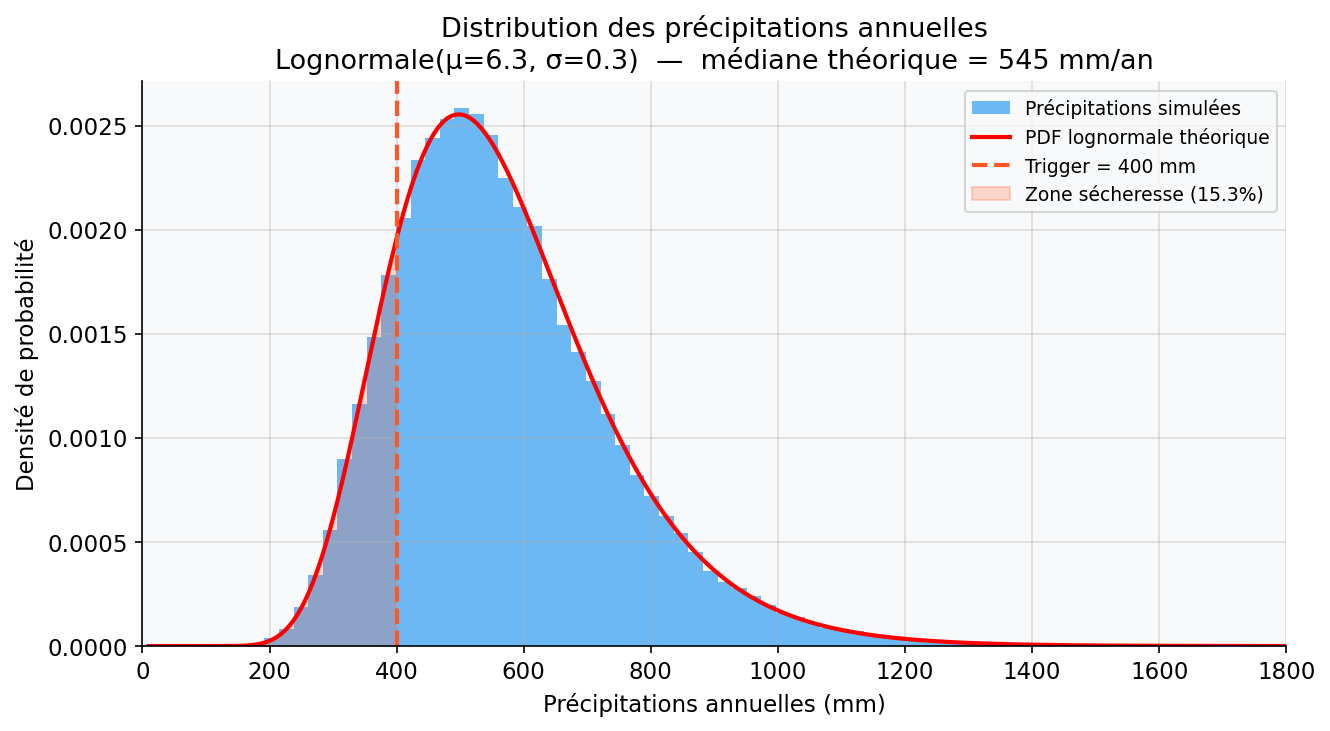
\includegraphics[width=\textwidth]{figures/01_distribution_precipitations.png}
      {\centering\footnotesize Distribution simulée ($N=100\,000$)\par}
  \end{columns}
\end{frame}

% ─────────────────────────────────────────────────────────────────────────────
\begin{frame}{Calcul de la probabilité de sécheresse}
  \begin{columns}[c]
    \column{0.52\textwidth}
      \textbf{Probabilité de déclenchement} $p$ :
      \[
        p = \mathbb{P}(X < 400) = \Phi\!\left(\frac{\ln 400 - \mu}{\sigma}\right)
      \]
      \[
        = \Phi\!\left(\frac{5{,}991 - 6{,}30}{0{,}30}\right)
        = \Phi(-1{,}03) \approx \mathbf{15{,}2\,\%}
      \]

      \begin{block}{Interprétation}
        \begin{itemize}
          \setlength{\itemsep}{3pt}
          \item Sécheresse déclencheuse $\approx$ \textbf{1 fois tous les 6--7 ans}
          \item Cohérent avec les observations historiques
          \item Test KS : $p = 0{,}048$ (déviation mineure, $N$ grand)
        \end{itemize}
      \end{block}

      \vspace{0.2em}
      \textbf{Validation Monte Carlo} ($N = 100\,000$) :\\
      $\hat{p} = 15{,}20\,\%$ vs $p_{\text{th}} = 15{,}19\,\%$ \quad \textcolor{SuccessGreen}{\faCheckCircle\ Validé}

    \column{0.45\textwidth}
      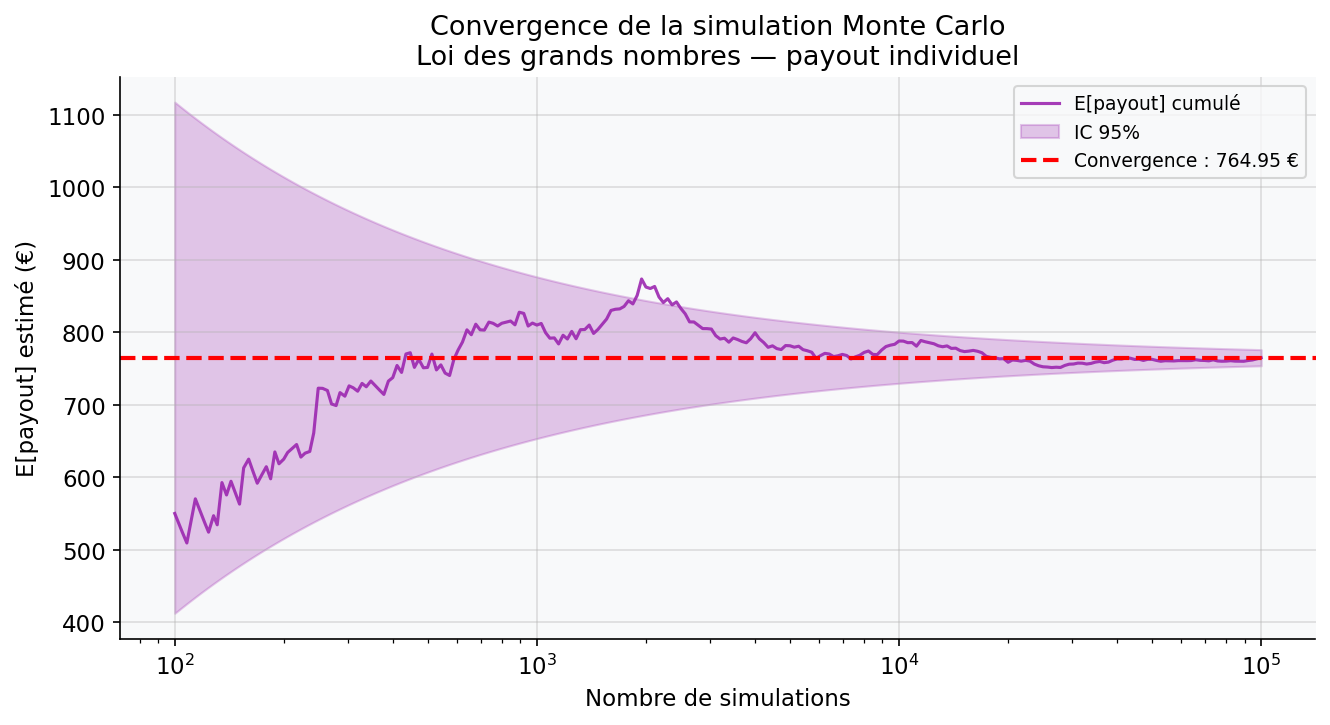
\includegraphics[width=\textwidth]{figures/02_convergence_monte_carlo.png}
      {\centering\footnotesize Convergence MC --- Loi des grands nombres\par}
  \end{columns}
\end{frame}

% ─────────────────────────────────────────────────────────────────────────────
\begin{frame}{Prime actuariellement équitable}
  \begin{columns}[c]
    \column{0.53\textwidth}
      \begin{block}{Tarification actuarielle}
        \[
          \pi_{\text{pure}} = p \cdot C
          = 15{,}2\% \times 5\,000 = \mathbf{760\,\text{\euro/an}}
        \]
        \vspace{-0.3em}
        \renewcommand{\arraystretch}{1.25}
        \begin{tabular}{@{}ll@{}}
          \toprule
          Prime commerciale $\pi_c$ & $\mathbf{950\,\text{\euro/an}}$ \\
          Chargement $\lambda$       & $25\,\%$ \\
          Loss Ratio                 & $\mathbf{80\,\%}$ \\
          IC 95\,\%                  & $[\,749\,;\,771\,]$\,\euro \\
          $\sigma[L]$                & $1\,795\,\text{\euro}$ \\
          \bottomrule
        \end{tabular}
      \end{block}
      \vspace{0.3em}
      \begin{exampleblock}{\small\faCalculator\ Formule}
        \small $\pi_c = \pi_{\text{pure}} \times (1 + \lambda) = 760 \times 1{,}25 = 950\,\text{\euro}$
      \end{exampleblock}
    \column{0.44\textwidth}
      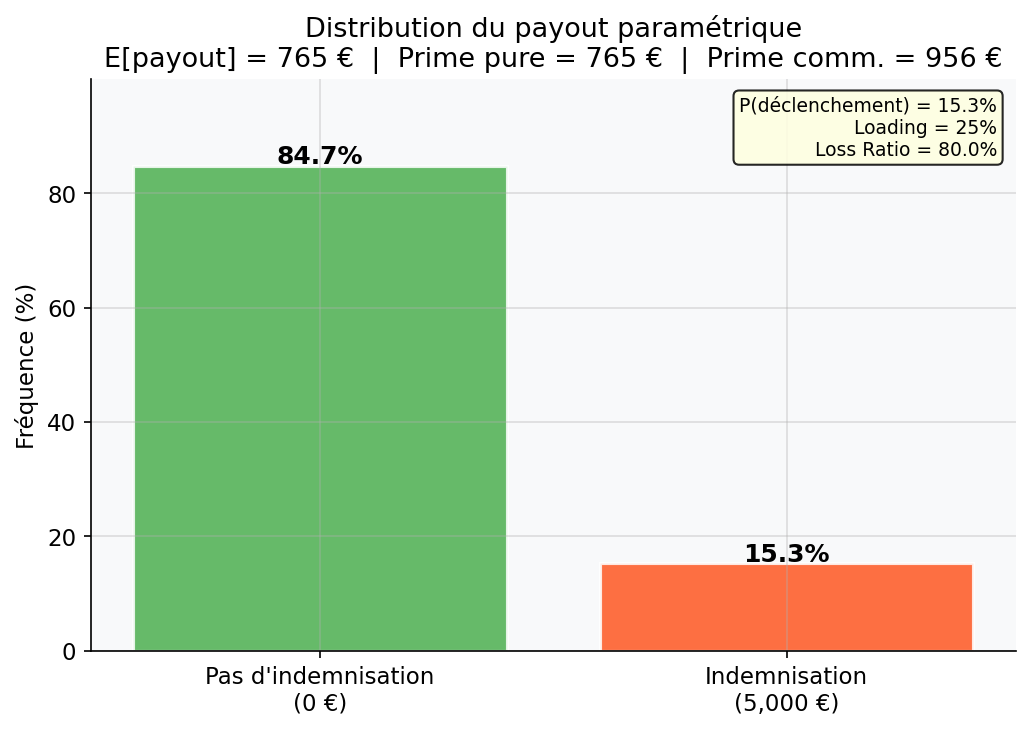
\includegraphics[width=\textwidth]{figures/03_distribution_payout.png}
      {\centering\footnotesize Distribution du payout binaire\par}
  \end{columns}
\end{frame}

% ══════════════════════════════════════════════════════════════════════════════
\section{Simulation Financière}
% ══════════════════════════════════════════════════════════════════════════════

\sectionslide{4. Simulation Financière}{Livrables 2 \& 5 --- Portefeuille, VaR, stress test, rentabilité}

% ─────────────────────────────────────────────────────────────────────────────
\begin{frame}{Rentabilité du portefeuille assureur --- Livrable 2 \& 5}
  \begin{columns}[c]
    \column{0.50\textwidth}
      \begin{block}{Paramètres portefeuille}
        \begin{itemize}
          \setlength{\itemsep}{3pt}
          \item $N = 500$ assurés, horizon 20 ans
          \item Primes collectées : $500 \times 950 = $ \textbf{475\,k\euro/an}
          \item Sinistres espérés : $500 \times 0{,}152 \times 5\,000 = $ \textbf{380\,k\euro/an}
          \item Profit moyen attendu : \textbf{$\approx$\,100\,k\euro/an}
        \end{itemize}
      \end{block}

      \begin{alertblock}{Mesures de risque (VaR / CVaR)}
        \small
        \renewcommand{\arraystretch}{1.25}
        \begin{tabular}{@{}lr@{}}
          VaR 95\,\% (perte nette) & $-$30\,k\euro \\
          VaR 99\,\% (perte nette) & $\approx\,0$\,\euro \\
          CVaR 99\,\%              & +\,9\,k\euro \\
          \textbf{P(déficit)}      & \textbf{0{,}89\,\%} \\
        \end{tabular}
      \end{alertblock}
    \column{0.47\textwidth}
      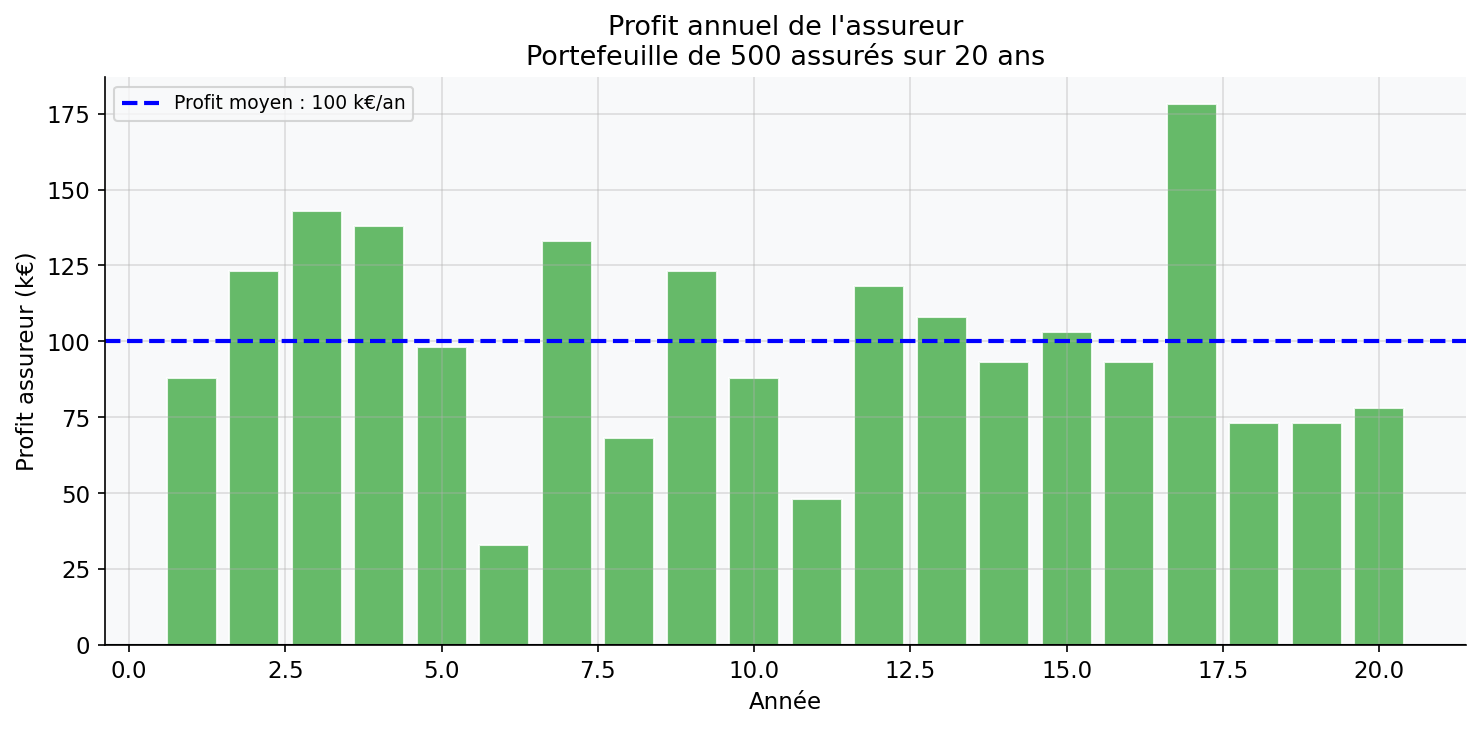
\includegraphics[width=\textwidth]{figures/05_profit_annuel_assureur.png}
      {\centering\footnotesize Profit annuel assureur (20 ans simulés)\par}
  \end{columns}
\end{frame}

% ─────────────────────────────────────────────────────────────────────────────
\begin{frame}{Distribution des pertes agrégées}
  \begin{columns}[c]
    \column{0.50\textwidth}
      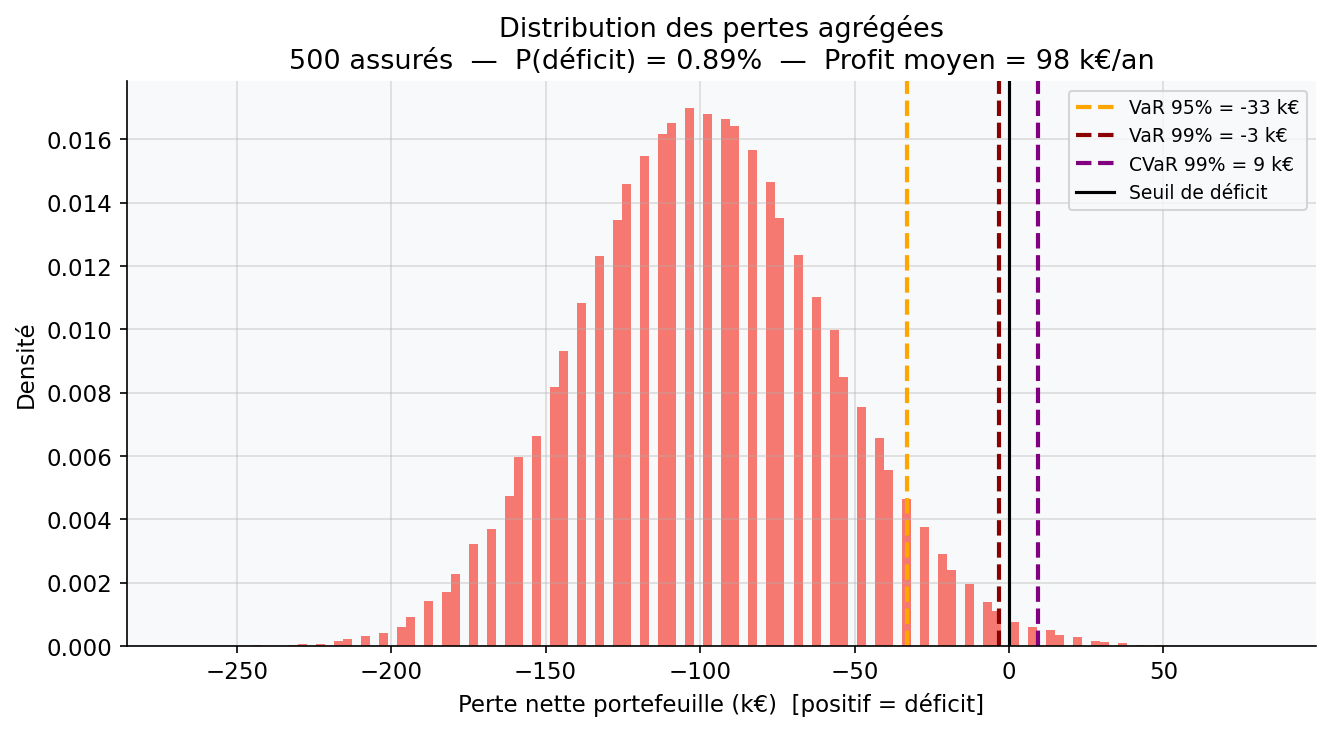
\includegraphics[width=\textwidth]{figures/04_distribution_pertes_portefeuille.png}
      {\centering\footnotesize Pertes nettes agrégées ($100\,000$ simulations)\par}
    \column{0.47\textwidth}
      \begin{block}{Lecture du graphique}
        \begin{itemize}
          \setlength{\itemsep}{4pt}
          \item La \textbf{grande majorité} des scénarios est profitable
          \item VaR 99\,\% $\approx 0$ : profit dans 99\,\% des cas
          \item Seule la queue extrême expose au déficit
        \end{itemize}
      \end{block}

      \begin{block}{Perspective de l'assuré}
        \begin{itemize}
          \setlength{\itemsep}{3pt}
          \item Gain net moyen sur 20 ans : \textbf{$-$3\,950\,\euro}
          \item = coût du loading cumulé
          \item \textbf{36\,\%} des assurés ont un gain positif
        \end{itemize}
        \vspace{0.2em}
        {\small\itshape L'assurance est un \textbf{transfert de risque}, pas un investissement.}
      \end{block}
  \end{columns}
\end{frame}

% ─────────────────────────────────────────────────────────────────────────────
\begin{frame}{Rentabilité : synthèse assureur vs assuré --- Livrable 5}
  \begin{columns}[t]
    \column{0.48\textwidth}
      \begin{block}{\faBuilding\ Perspective assureur}
        \renewcommand{\arraystretch}{1.2}
        \small
        \begin{tabular}{@{}ll@{}}
          Primes / an       & 475\,k\euro \\
          Sinistres esp.    & 380\,k\euro \\
          \textbf{Profit moy.} & \textbf{100\,k\euro/an} \\
          P(déficit)        & 0{,}89\,\% \\
          Années déf. / 20  & 0 \\
        \end{tabular}

        \vspace{0.3em}
        \textcolor{SuccessGreen}{\faCheckCircle}\ Modèle \textbf{rentable} et stable\\
        \textcolor{SuccessGreen}{\faCheckCircle}\ Coûts admin. réduits ($-70\,\%$)\\
        \textcolor{WarnOrange}{\faExclamationTriangle}\ Risque systémique (sécheresse nationale)
      \end{block}
    \column{0.48\textwidth}
      \begin{block}{\faUser\ Perspective assuré}
        \renewcommand{\arraystretch}{1.2}
        \small
        \begin{tabular}{@{}ll@{}}
          Prime / an        & 950\,\euro \\
          Payout si décl.   & 5\,000\,\euro \\
          \textbf{Gain net / 20 ans} & \textbf{$-$3\,950\,\euro} \\
          \% gain positif   & 36\,\% \\
          Coût loading / an & 197\,\euro \\
        \end{tabular}

        \vspace{0.3em}
        \textcolor{SuccessGreen}{\faCheckCircle}\ Paiement \textbf{garanti} (code immuable)\\
        \textcolor{SuccessGreen}{\faCheckCircle}\ Règlement $<$ 1 minute\\
        \textcolor{WarnOrange}{\faExclamationTriangle}\ Gain net négatif en espérance
      \end{block}
  \end{columns}
\end{frame}

% ─────────────────────────────────────────────────────────────────────────────
\begin{frame}{Stress test climatique --- Livrable 2}
  \begin{columns}[c]
    \column{0.60\textwidth}
      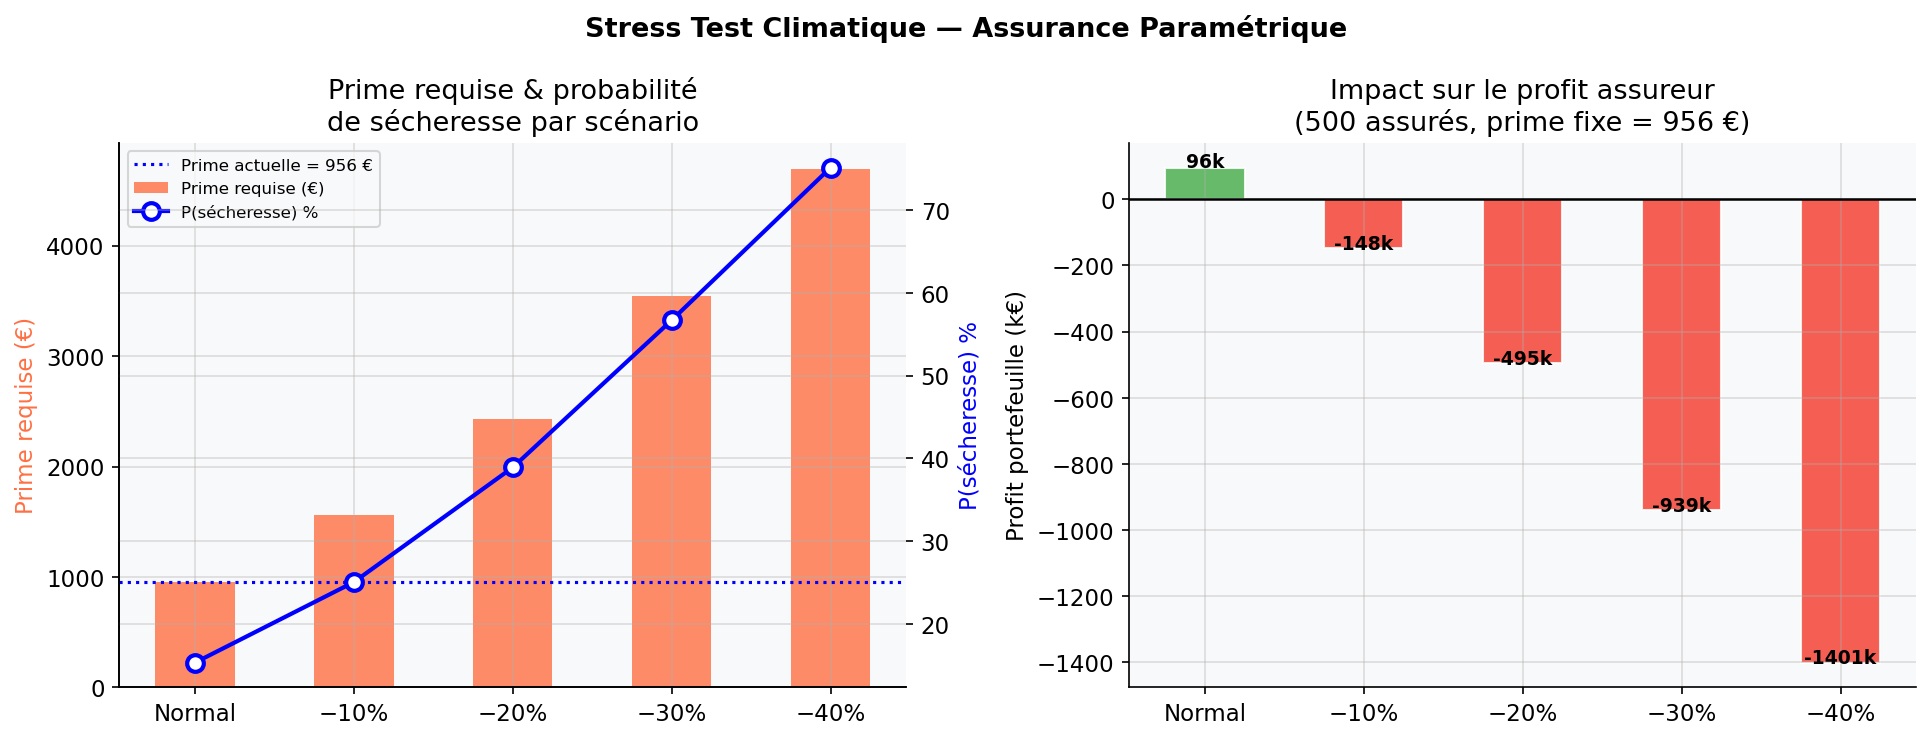
\includegraphics[width=\textwidth]{figures/08_stress_test.png}
      {\centering\footnotesize Impact des scénarios de stress sur la prime et le profit\par}
    \column{0.37\textwidth}
      \begin{alertblock}{Résultats clés}
        \small
        \renewcommand{\arraystretch}{1.3}
        \begin{tabular}{@{}lcc@{}}
          \toprule
          Scénario & $p$ & Prime \\
          \midrule
          Normal   & 15\,\% & 950\,\euro \\
          $-10\,\%$& 25\,\% & 1\,565\,\euro \\
          $-20\,\%$& 39\,\% & 2\,430\,\euro \\
          $-30\,\%$& 57\,\% & 3\,540\,\euro \\
          \bottomrule
        \end{tabular}
      \end{alertblock}
      \begin{alertblock}{\small \faExclamationTriangle\ Conclusion}
        \small
        Un scénario $-30\,\%$ (compatible GIEC RCP\,8.5 pour le bassin méditerranéen à horizon 2050) rend le produit \textbf{non viable} sans révision tarifaire dynamique.
      \end{alertblock}
  \end{columns}
\end{frame}

% ══════════════════════════════════════════════════════════════════════════════
\section{Risque Moral \& Oracles}
% ══════════════════════════════════════════════════════════════════════════════

\sectionslide{5. Analyse des Risques}{Livrables 3 \& 4 --- Risque moral, oracles, basis risk}

% ─────────────────────────────────────────────────────────────────────────────
\begin{frame}{Analyse du risque moral --- Livrable 3}
  \begin{columns}[t]
    \column{0.48\textwidth}
      \begin{alertblock}{Assurance traditionnelle}
        \begin{itemize}
          \setlength{\itemsep}{4pt}
          \item[\textcolor{AlertRed}{\faTimesCircle}] \textbf{Ex ante} : moindre prévention
          \item[\textcolor{AlertRed}{\faTimesCircle}] \textbf{Ex post} : déclaration exagérée
          \item[\textcolor{AlertRed}{\faTimesCircle}] Collusion expert-assuré
          \item[\textcolor{AlertRed}{\faTimesCircle}] Fraude à l'expertise
        \end{itemize}
      \end{alertblock}
    \column{0.48\textwidth}
      \begin{exampleblock}{Paramétrique blockchain}
        \begin{itemize}
          \setlength{\itemsep}{4pt}
          \item[\textcolor{SuccessGreen}{\faCheckCircle}] Trigger \textbf{objectif} (météo)
          \item[\textcolor{SuccessGreen}{\faCheckCircle}] Aucune déclaration humaine
          \item[\textcolor{SuccessGreen}{\faCheckCircle}] Oracle = tiers mécanique impartial
          \item[\textcolor{WarnOrange}{\faExclamationTriangle}] Sélection adverse résiduelle
        \end{itemize}
      \end{exampleblock}
  \end{columns}

  \vspace{0.3em}
  \begin{block}{\faKey\ Mécanisme d'élimination du risque moral}
    \small
    Le payout est déclenché par une variable météorologique
    \textbf{indépendante des actions de l'agriculteur}.
    Il est physiquement impossible d'influencer la pluviométrie d'une région
    $\Rightarrow$ le risque moral ex post est \textbf{structurellement éliminé}.
  \end{block}

  \vspace{0.2em}
  \begin{columns}[t]
    \column{0.48\textwidth}
      \begin{alertblock}{\small Risque moral résiduel}
        \small\warn{} Choix de cultures plus risquées (couverture disponible)
      \end{alertblock}
    \column{0.48\textwidth}
      \begin{alertblock}{\small Sélection adverse}
        \small\warn{} Zones à fort risque surreprésentées dans le portefeuille
      \end{alertblock}
  \end{columns}
\end{frame}

% ─────────────────────────────────────────────────────────────────────────────
\begin{frame}{Les oracles : fiabilité \& manipulation --- Livrable 4}
  \begin{columns}[c]
    \column{0.52\textwidth}
      \begin{block}{Le problème de l'oracle}
        \small
        Un smart contract ne peut accéder qu'aux données \textbf{on-chain}.
        L'oracle est le \textbf{pont} entre le monde réel et la blockchain.\\[4pt]
        \textcolor{AlertRed}{\itshape Si l'oracle est corruptible, toute la sécurité du contrat s'effondre.}
      \end{block}

      \vspace{0.3em}
      \textbf{Solution : Chainlink DON}

      \begin{tikzpicture}[scale=0.78, every node/.style={font=\tiny},
          box/.style={draw, rounded corners, minimum height=0.5cm, text centered}]
        \node[box, fill=orange!20, minimum width=1.5cm] (noaa) at (0,1.5) {NOAA};
        \node[box, fill=orange!20, minimum width=1.5cm] (omet) at (2,1.5) {Open-Meteo};
        \node[box, fill=orange!20, minimum width=1.5cm] (era) at (4,1.5) {ERA5};
        \node[box, fill=AccentBlue!25, minimum width=3.8cm] (agg) at (2,0.7) {Agrégation --- médiane};
        \node[box, fill=LightBlue, minimum width=3.8cm] (sc2) at (2,0) {\faCode\ Smart Contract};
        \draw[-{Stealth}] (noaa) -- (agg);
        \draw[-{Stealth}] (omet) -- (agg);
        \draw[-{Stealth}] (era) -- (agg);
        \draw[-{Stealth}] (agg) -- (sc2);
      \end{tikzpicture}

    \column{0.45\textwidth}
      \small
      \renewcommand{\arraystretch}{1.25}
      \begin{tabular}{@{}p{2.0cm}p{2.7cm}@{}}
        \toprule
        \textbf{Attaque} & \textbf{Mitigation} \\
        \midrule
        1 node corrompu & Médiane de $N$ nodes \\
        Collusion & Staking LINK (slashing) \\
        Station biaisée & Multi-sources croisées \\
        Données périmées & \texttt{\scriptsize ORACLE\_MAX\_AGE} \\
        Replay attack & Vérif. timestamp \\
        \bottomrule
      \end{tabular}

      \vspace{0.4em}
      \begin{alertblock}{\small Limites résiduelles}
        \small
        Indisponibilité réseau, délai de mise à jour, coût opérationnel (tokens LINK).
      \end{alertblock}
  \end{columns}
\end{frame}

% ══════════════════════════════════════════════════════════════════════════════
\section{Basis Risk \& Limites}
% ══════════════════════════════════════════════════════════════════════════════

% ─────────────────────────────────────────────────────────────────────────────
\begin{frame}{Le basis risk : principale limite du modèle}
  \begin{columns}[c]
    \column{0.50\textwidth}
      \begin{alertblock}{Définition}
        Le \textbf{basis risk} est l'écart entre la perte réelle
        de l'agriculteur et l'indemnisation reçue :
        \[
          BR = \underbrace{L_{\text{réelle}}}_{\text{parcelle}} - \underbrace{\text{Payout}}_{\text{station oracle}}
        \]
      \end{alertblock}

      \vspace{0.2em}
      \textbf{Modèle bivarié lognormal} ($\rho = 0{,}75$) :
      \[
        \ln X_{\text{parcelle}} = \rho \cdot Z_s + \sqrt{1-\rho^2}\,\varepsilon
      \]

      \begin{block}{Résultats ($N = 50\,000$)}
        \renewcommand{\arraystretch}{1.2}
        \begin{tabular}{@{}ll@{}}
          $\sigma(BR)$       & $\mathbf{1\,870}$\,\euro \\
          Sous-assurés       & \textbf{6{,}7\,\%} \\
          Sur-indemnisés     & \textbf{6{,}7\,\%} \\
        \end{tabular}
      \end{block}

    \column{0.47\textwidth}
      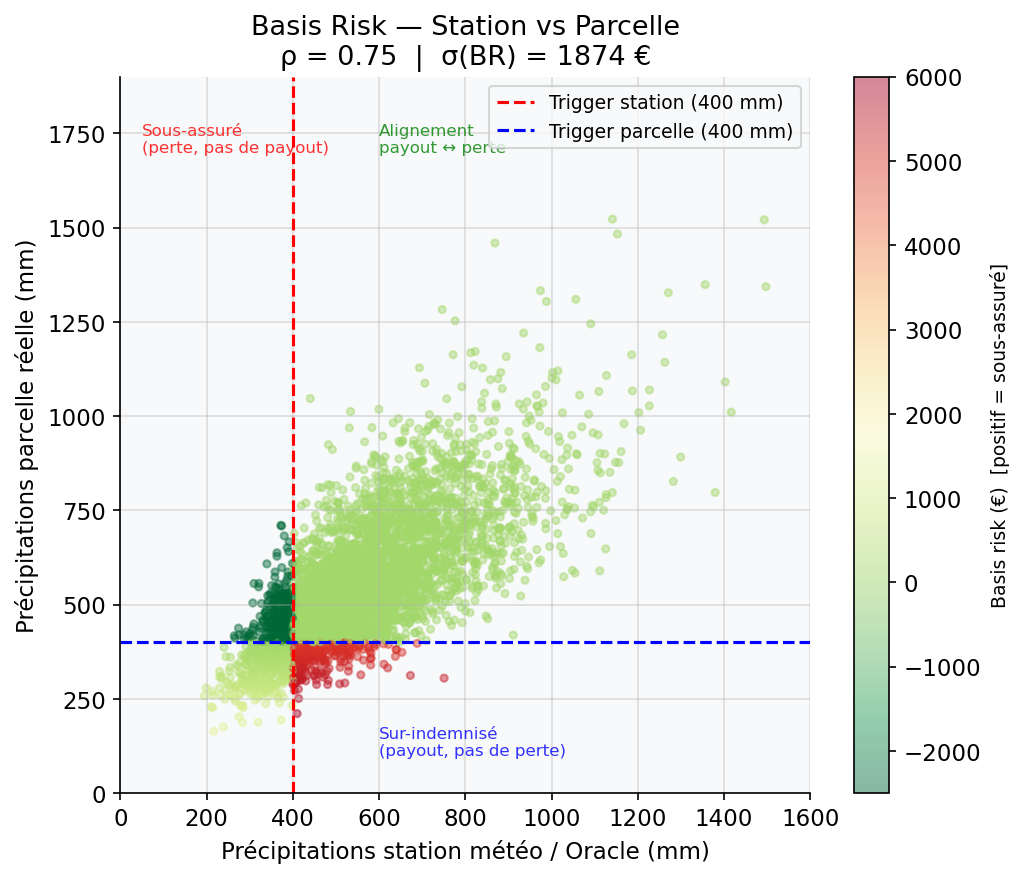
\includegraphics[width=\textwidth]{figures/10_basis_risk_scatter.png}
      {\centering\footnotesize Station vs Parcelle --- coloration par basis risk\par}
  \end{columns}
\end{frame}

% ─────────────────────────────────────────────────────────────────────────────
\begin{frame}{Basis risk : distribution \& sensibilité à $\rho$}
  \begin{columns}[c]
    \column{0.48\textwidth}
      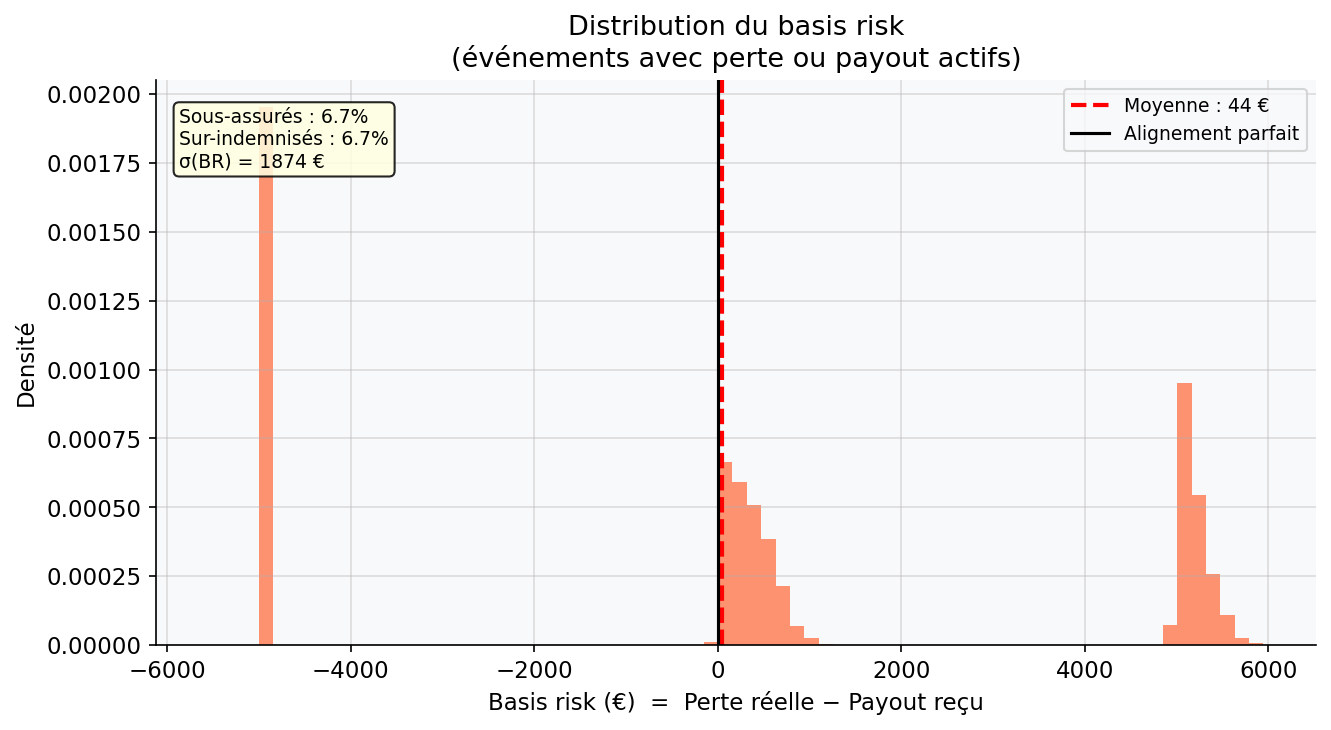
\includegraphics[width=\textwidth]{figures/11_basis_risk_distribution.png}
      {\centering\footnotesize Distribution du basis risk (événements actifs)\par}
    \column{0.48\textwidth}
      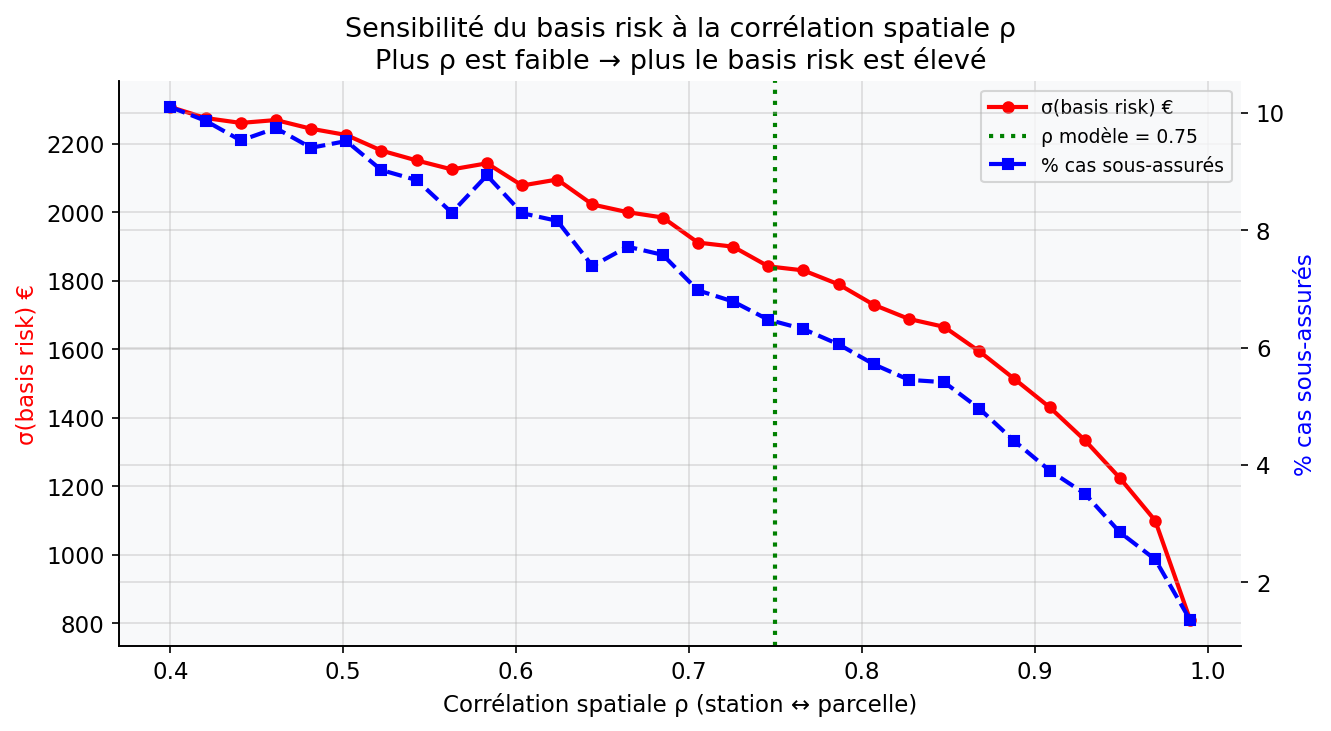
\includegraphics[width=\textwidth]{figures/12_basis_risk_sensibilite.png}
      {\centering\footnotesize Sensibilité à la corrélation spatiale $\rho$\par}
  \end{columns}

  \vspace{0.3em}
  \begin{exampleblock}{Pistes de réduction du basis risk}
    \begin{multicols}{2}
      \begin{itemize}
        \setlength{\itemsep}{2pt}
        \item Réseau dense de stations IoT
        \item Données satellitaires (NDVI, Sentinel-2)
        \item Trigger multi-indicateurs (pluie + NDVI)
        \item Micro-zonage régional adaptatif
      \end{itemize}
    \end{multicols}
  \end{exampleblock}
\end{frame}

% ─────────────────────────────────────────────────────────────────────────────
\begin{frame}{Limites réglementaires}
  \begin{columns}[c]
    \column{0.55\textwidth}
      \begin{alertblock}{Obstacles juridiques en France}
        \begin{itemize}
          \setlength{\itemsep}{6pt}
          \item[\textcolor{AlertRed}{\faGavel}] Smart contracts \textbf{non reconnus}
            par le Code des assurances français
          \item[\textcolor{AlertRed}{\faUniversity}] \textbf{Solvabilité II} :
            exigences de capital incompatibles avec les réserves on-chain
          \item[\textcolor{AlertRed}{\faIdCard}] \textbf{KYC/AML} :
            pseudonymat blockchain vs. identification obligatoire
          \item[\textcolor{AlertRed}{\faUserShield}] \textbf{RGPD} :
            données immuables vs. droit à l'effacement (art. 17)
        \end{itemize}
      \end{alertblock}
    \column{0.42\textwidth}
      \begin{exampleblock}{\small\faLightbulb\ Pistes}
        \small
        \begin{itemize}
          \setlength{\itemsep}{4pt}
          \item Cadre \textbf{sandbox réglementaire} (ACPR)
          \item Blockchain permissionnée (Hyperledger)
          \item Données chiffrées off-chain + hash on-chain
          \item Partenariat avec un assureur agréé
        \end{itemize}
      \end{exampleblock}
  \end{columns}
\end{frame}

% ─────────────────────────────────────────────────────────────────────────────
\begin{frame}{Limites actuarielles \& techniques}
  \begin{columns}[c]
    \column{0.55\textwidth}
      \begin{alertblock}{Fragilités du modèle}
        \begin{itemize}
          \setlength{\itemsep}{6pt}
          \item[\textcolor{AlertRed}{\faTemperatureHigh}] Distribution \textbf{non stationnaire} :
            le changement climatique invalide à terme la calibration historique
          \item[\textcolor{AlertRed}{\faProjectDiagram}] \textbf{Corrélation spatiale} :
            une sécheresse nationale touche tout le portefeuille simultanément
          \item[\textcolor{AlertRed}{\faExchangeAlt}] \textbf{Volatilité ETH} :
            prime en crypto $\neq$ valeur \euro{} fixe au moment du payout
          \item[\textcolor{AlertRed}{\faWallet}] \textbf{Accessibilité} :
            wallet crypto complexe pour les exploitants agricoles
        \end{itemize}
      \end{alertblock}
    \column{0.42\textwidth}
      \begin{exampleblock}{\small\faLightbulb\ Solutions proposées}
        \small
        \begin{itemize}
          \setlength{\itemsep}{4pt}
          \item Prime en \textbf{stablecoin} (USDC/DAI)
          \item Indice NDVI via Sentinel-2
          \item Modèle de prime \textbf{dynamique} recalibré annuellement
          \item \textbf{Réassurance on-chain} (CAT bonds tokenisés)
          \item Interface mobile simplifiée
        \end{itemize}
      \end{exampleblock}
  \end{columns}
\end{frame}

% ══════════════════════════════════════════════════════════════════════════════
\section{Synthèse \& Conclusion}
% ══════════════════════════════════════════════════════════════════════════════

\sectionslide{Synthèse \& Conclusion}{Bilan, résultats clés et perspectives}

% ─────────────────────────────────────────────────────────────────────────────
\begin{frame}{Bilan de la simulation}
  \begin{columns}[c]
    \column{0.52\textwidth}
      \renewcommand{\arraystretch}{1.30}
      \begin{tabular}{@{}lc@{}}
        \toprule
        \textbf{Indicateur} & \textbf{Valeur} \\
        \midrule
        P(sécheresse) & 15{,}2\,\% \\
        Prime pure & 760\,\euro/an \\
        IC 95\,\% prime & [749 ; 771] \\
        Prime commerciale & 950\,\euro/an \\
        Loss Ratio & 80\,\% \\
        \midrule
        Profit assureur/an & $\approx$100\,k\euro \\
        P(déficit) & \textbf{0{,}89\,\%} \\
        CVaR 99\,\% & 9\,k\euro \\
        \midrule
        $\sigma$(basis risk) & 1\,870\,\euro \\
        Test KS & p\,=\,0{,}048 \\
        Simulations MC & $N = 100\,000$ \\
        \bottomrule
      \end{tabular}
    \column{0.45\textwidth}
      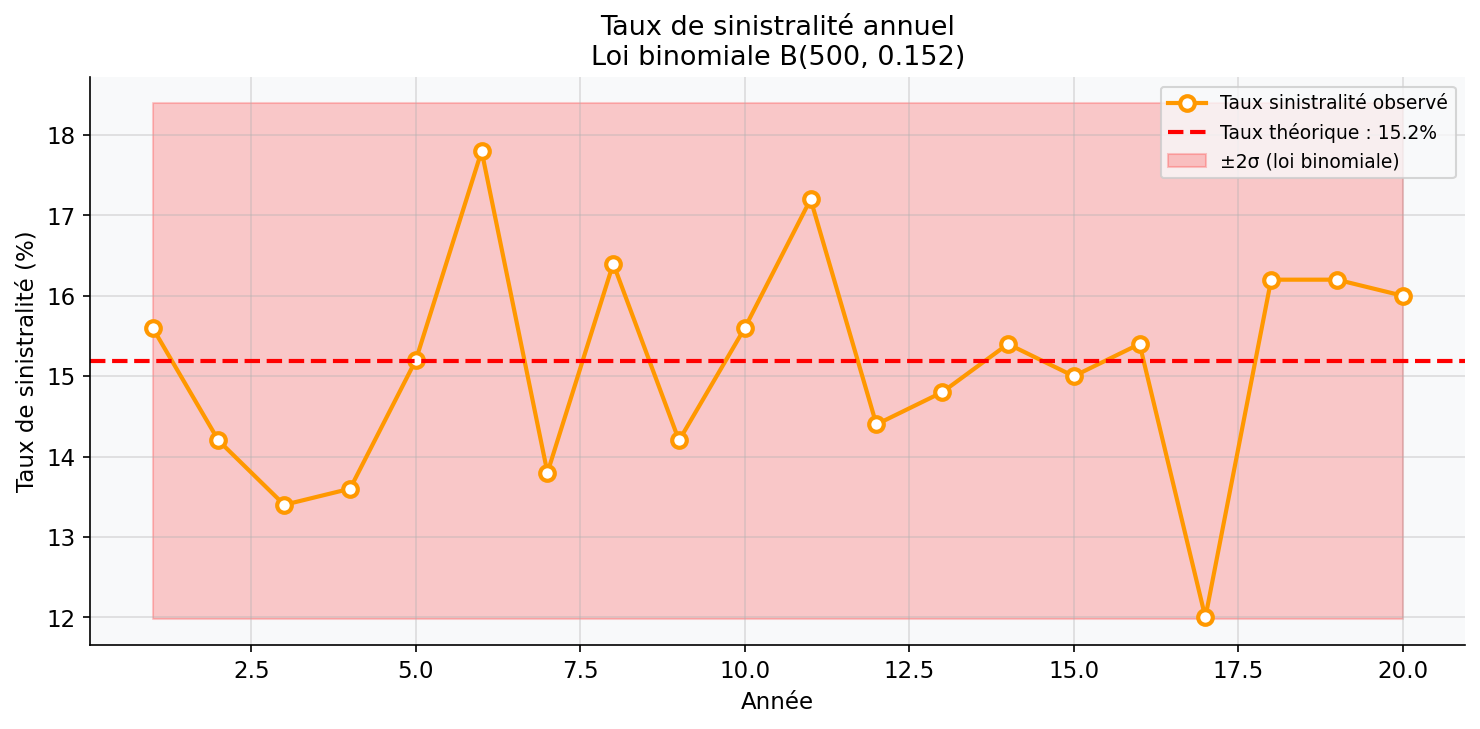
\includegraphics[width=\textwidth]{figures/06_taux_sinistralite.png}
      {\centering\footnotesize Taux sinistralité observé vs théorique\par}
  \end{columns}
\end{frame}

% ─────────────────────────────────────────────────────────────────────────────
\begin{frame}{Conclusion}
  \begin{block}{Ce que nous avons démontré}
    \begin{itemize}
      \setlength{\itemsep}{4pt}
      \item[\good{}] La modélisation lognormale est \textbf{calibrée et validée} ($p = 15{,}2\,\%$, KS OK)
      \item[\good{}] La prime de \textbf{950\,\euro/an} est actuariellement équitable (LR = 80\,\%)
      \item[\good{}] Le portefeuille est \textbf{rentable} sur 20 ans avec P(déficit) $<\,1\,\%$
      \item[\good{}] Le risque moral est \textbf{structurellement éliminé} par le mécanisme paramétrique
      \item[\warn{}] Le basis risk ($\sigma \approx 1\,870$\,\euro) reste la \textbf{limite principale}
      \item[\warn{}] Le stress test révèle une \textbf{forte sensibilité} au changement climatique
    \end{itemize}
  \end{block}

  \begin{exampleblock}{Message central}
    \centering
    \textit{Les smart contracts n'éliminent pas l'actuariat ---
    ils l'\textbf{automatisent} et l'\textbf{objectivent}.\\[3pt]
    La vraie valeur réside dans la \textbf{réduction des coûts de transaction}
    et l'\textbf{élimination des asymétries d'information}.}
  \end{exampleblock}
\end{frame}

% ─────────────────────────────────────────────────────────────────────────────
\begin{frame}{Ouverture : vers un produit déployable~?}
  \begin{columns}[t]
    \column{0.48\textwidth}
      \begin{block}{\faRocket\ Court terme (faisable)}
        \begin{itemize}
          \setlength{\itemsep}{4pt}
          \item Déploiement sur testnet Polygon (faibles frais gas)
          \item Prime en stablecoin USDC
          \item Intégration Chainlink Automation pour déclenchement automatique
          \item Interface mobile simplifiée (abstraction de wallet)
        \end{itemize}
      \end{block}
    \column{0.48\textwidth}
      \begin{block}{\faFlask\ Moyen terme (recherche)}
        \begin{itemize}
          \setlength{\itemsep}{4pt}
          \item Trigger \textbf{multi-indicateurs} : pluie + NDVI + température
          \item \textbf{Prime dynamique} recalibrée avec données satellite temps réel
          \item \textbf{Réassurance on-chain} via CAT bonds tokenisés (ERC-20)
          \item Pool de liquidité mutualisée inter-régions
        \end{itemize}
      \end{block}
  \end{columns}
  \vspace{0.4em}
  \begin{alertblock}{\small\faGavel\ Condition sine qua non}
    \small\centering
    Le déploiement commercial nécessite un \textbf{cadre réglementaire adapté}
    (sandbox ACPR) ou un partenariat avec un assureur agréé Code des assurances.
  \end{alertblock}
\end{frame}

% ─────────────────────────────────────────────────────────────────────────────
% SLIDE FINALE — QUESTIONS
% ─────────────────────────────────────────────────────────────────────────────
\begin{frame}[plain]
  \begin{tikzpicture}[remember picture, overlay]
    \fill[MainBlue] (current page.south west) rectangle (current page.north east);
    \node[white, font=\Huge\bfseries] at ($(current page.center)+(0,1.2)$)
      {Merci de votre attention};
    \draw[white, line width=2pt]
      ($(current page.center)+(-5,0.3)$) -- ($(current page.center)+(5,0.3)$);
    \node[white, font=\Large] at ($(current page.center)+(0,-0.5)$)
      {\faQuestionCircle\quad Questions~?};
    \node[white!70, font=\small] at ($(current page.center)+(0,-1.5)$)
      {Rania \textsc{Wahbi} · Antoine \textsc{Serac} · Louis \textsc{Jeaate}};
    \node[white!50, font=\footnotesize] at ($(current page.center)+(0,-2.2)$)
      {ECE Paris --- ING4 FIQ --- 2025--2026};
  \end{tikzpicture}
\end{frame}


% ══════════════════════════════════════════════════════════════════════════════
% ANNEXES
% ══════════════════════════════════════════════════════════════════════════════
\appendix

\begin{frame}{Annexe A --- Comparaison paramétrique vs traditionnelle}
  \begin{columns}[c]
    \column{0.50\textwidth}
      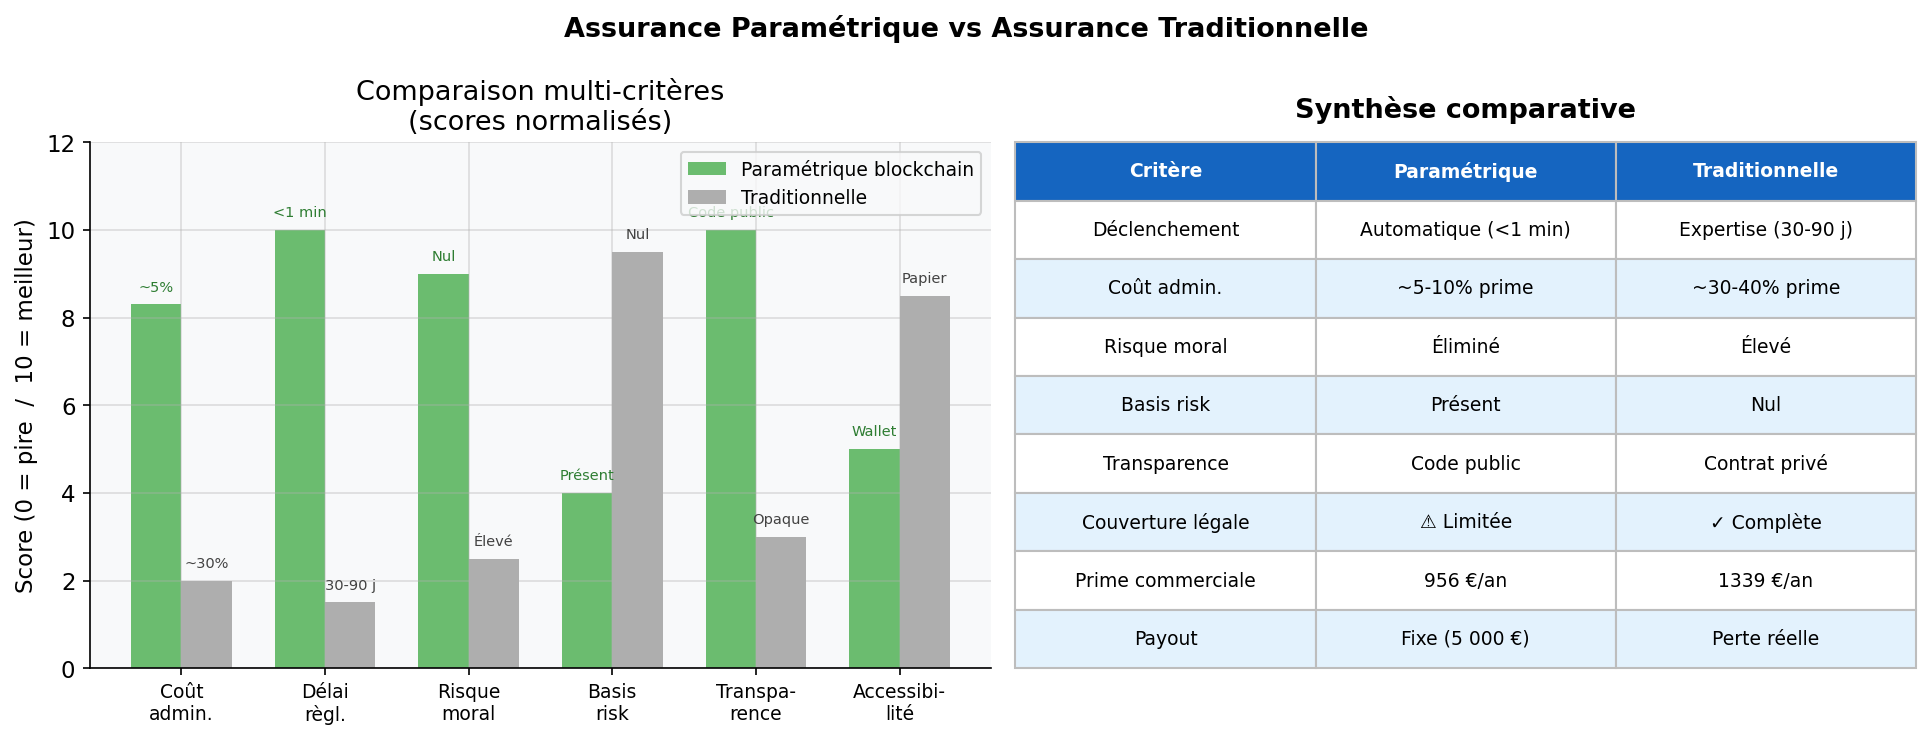
\includegraphics[width=\textwidth]{figures/09_comparaison_param_vs_trad.png}
      {\centering\footnotesize Scores multi-critères normalisés\par}
    \column{0.47\textwidth}
      \small
      \renewcommand{\arraystretch}{1.15}
      \begin{tabular}{@{}lcc@{}}
        \toprule
        \textbf{Critère} & \textbf{Param.} & \textbf{Trad.} \\
        \midrule
        Déclenchement & Auto ($<$1 min) & 30--90 j \\
        Coût admin.   & 5--10\,\%       & 30--40\,\% \\
        Risque moral  & Éliminé         & Élevé \\
        Basis risk    & Présent         & Nul \\
        Transparence  & Code public     & Contrat privé \\
        Cadre légal   & \warn{} Limité  & \good{} Complet \\
        \bottomrule
      \end{tabular}
  \end{columns}
\end{frame}

\begin{frame}{Annexe B --- Gain net de l'assuré}
  \begin{columns}[c]
    \column{0.52\textwidth}
      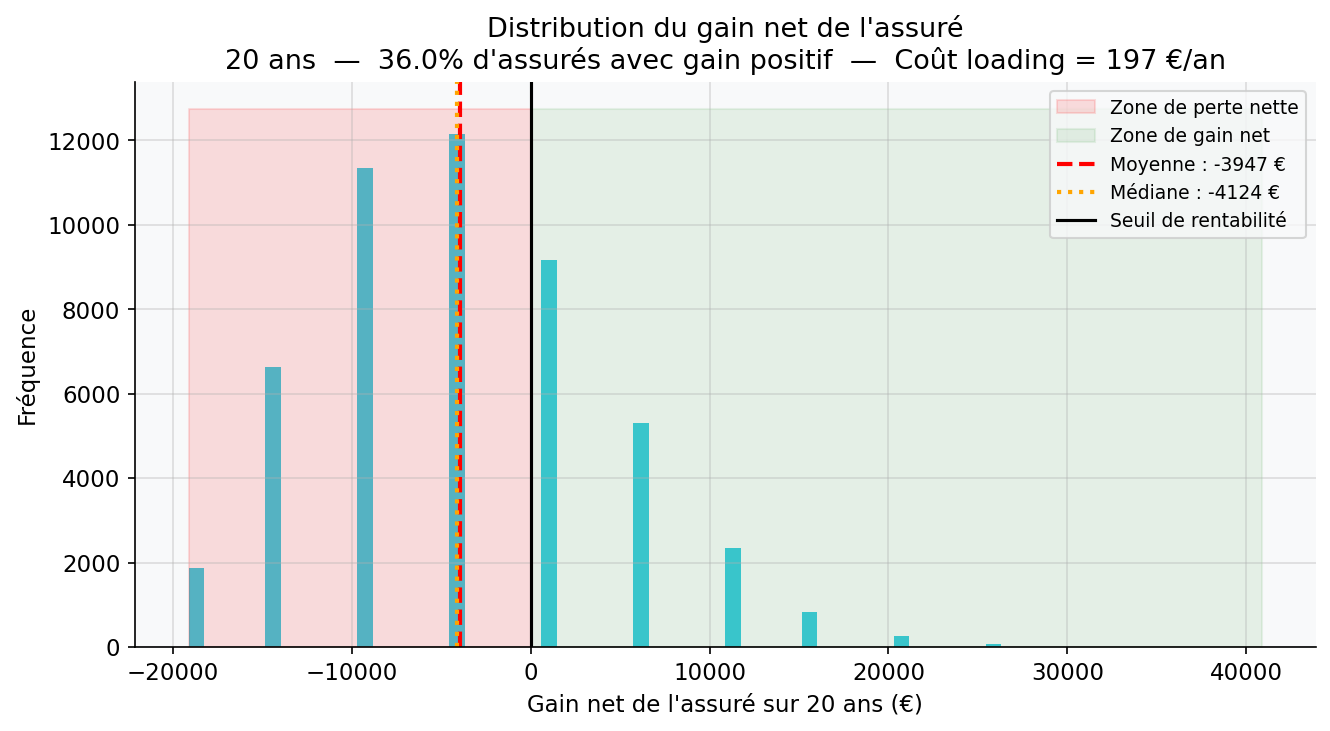
\includegraphics[width=\textwidth]{figures/07_gain_net_assure.png}
      {\centering\footnotesize Distribution du gain net assuré sur 20 ans ($N=50\,000$ sim.)\par}
    \column{0.45\textwidth}
      \begin{block}{Interprétation}
        \begin{itemize}
          \setlength{\itemsep}{3pt}
          \item Gain net moyen : \textbf{$-$3\,950\,\euro}
          \item $=$ coût du chargement 25\,\% sur 20 ans
          \item \textbf{36\,\%} des assurés ont un gain positif
          \item L'assurance est un \textbf{transfert de risque}, pas un investissement
          \item Valeur : lisser le revenu intertemporel de l'exploitant
        \end{itemize}
      \end{block}
  \end{columns}
\end{frame}

\begin{frame}{Annexe C --- Structure du code Python}
  \begin{block}{Architecture modulaire}
    \begin{columns}[t]
      \column{0.48\textwidth}
        \texttt{simulation/}
        \begin{itemize}
          \setlength{\itemsep}{2pt}
          \item \texttt{main.py} --- orchestration
          \item \texttt{src/config.py} --- paramètres centralisés
          \item \texttt{src/climate.py} --- scénarios climatiques
          \item \texttt{src/actuarial.py} --- prime, VaR, IC
          \item \texttt{src/portfolio.py} --- rentabilité, stress
          \item \texttt{src/basis\_risk.py} --- basis risk
          \item \texttt{src/plots.py} --- 12 graphiques
        \end{itemize}
      \column{0.48\textwidth}
        \texttt{results/}
        \begin{itemize}
          \item \texttt{figures/} --- 12 PNG
          \item \texttt{data/resultats\_annuels.csv}
        \end{itemize}
        \vspace{0.5em}
        \begin{exampleblock}{\small Lancement}
          \texttt{cd simulation \&\& python main.py}
        \end{exampleblock}
        \vspace{0.3em}
        \begin{block}{\small Stack}
          \small NumPy · SciPy · Matplotlib · Pandas
        \end{block}
    \end{columns}
  \end{block}
\end{frame}

\begin{frame}{Annexe D --- Références}
  \footnotesize
  \begin{itemize}
    \setlength{\itemsep}{3pt}
    \item \textbf{Fornier, Y.} (2024--2025). \textit{Comprendre la Blockchain --- Cours 4 : Les Smart Contracts}. ECE Paris
    \item Nakamoto, S. (2008). \textit{Bitcoin: A Peer-to-Peer Electronic Cash System}
    \item Szabo, N. (1997). \textit{Formalizing and Securing Relationships on Public Networks}
    \item Jensen, N.D., Barrett, C.B. (2017). \textit{Agricultural Index Insurance for Development}. Annual Review of Resource Economics
    \item Barnett, B.J., Mahul, O. (2007). \textit{Weather Index Insurance for Agriculture}. Am. J. of Agricultural Economics
    \item Chow, V.T. (1954). \textit{The log-probability law and its engineering applications}
    \item Chainlink Labs. \textit{Decentralized Oracle Networks}. \texttt{docs.chain.link}
    \item AXA Fizzy (2017). \textit{First blockchain-based flight-delay insurance}
    \item OpenZeppelin. \textit{Smart Contract Security Best Practices}. \texttt{docs.openzeppelin.com}
    \item GIEC / IPCC (2021). \textit{Sixth Assessment Report --- WGI}. Projections méditerranéennes RCP\,8.5
  \end{itemize}
\end{frame}

\end{document}
